\section{Grundlagen}

\begin{defi}{Anforderungen an Datenbanksysteme}
    \begin{itemize}
        \item Widerspruchsfreie, dauerhafte, effiziente und schnelle Speicherung von Daten jeder Art
        \item Bedarfsgerechte und optimierte Bereitstellung von Daten
        \item Datensicherheit und Datenschutz
        \item Mehrbenutzungsbetrieb
    \end{itemize}
\end{defi}

\begin{defi}{Datenbanksystem}
    Ein \emph{Datenbanksystem (DBS)} besteht aus dem Datenbankmanagementsystem (DBMS) und der Datenbank.
\end{defi}

\begin{defi}{Datenbankmanagementsystem}
    Ein \emph{Datenbankmanagementsystem (DBMS)} ist eine Software zur sicheren, konsistenten und persistenten Speicherung großer Datenmengen, mit dem Ziel mehreren Benutzern (gleichzeitig) effizienten, zuverlässigen, sicheren und bequemen Zugriff auf diese Daten zu ermöglichen.

    Es besteht aus Komponenten zur Abfrage, Verwaltung und Administration der Daten bzw. Datenbank.
\end{defi}

\begin{bonus}{DBMS Typen}
    Je nach Art der Daten und des Anwendungsfalls eignen sich unterschiedliche Typen von DBS, genauer DBMS, unterschiedlich gut.
    Da sind beispielsweise
    \begin{itemize}
        \item \emph{relationale DBMS}, die Objekten gleicher Struktur (Attribute) in Tabellen verwalten.
              \begin{itemize}
                  \item meist genutzt
                  \item SQL als Abfragesprache
                  \item vergleichsweise einfache und effiziente Behandlung von Objekten gleichen Aufbaus in Tabellen
                  \item in der Praxis sind viele Daten strukturiert und typisiert
              \end{itemize}
        \item \emph{hierarchische oder objektorientierte DBMS}, die Objekte mit Eltern-Kind- oder Vererbungsbeziehungen besitzen und einzelne Strukturen gemeinsam haben.
        \item \emph{dokumentenorientierte DBMS}, die Objekte ohne vergleichbare Strukturen verwalten.
    \end{itemize}
\end{bonus}

\begin{bonus}{Datum}
    \emph{Daten} sind zunächst Folgen von Zeichen (Zahlen, Buchstaben, Symbole) oder auch strukturierte Objekte.
    Sie folgen einer bestimmten Syntax.
\end{bonus}

\begin{bonus}{Information}
    Aus Daten entstehen \emph{Informationen}, wenn die Bedeutung bekannt ist.

    Durch die Hinzunahme von Semantik, ggf. weiteren Daten, kann das ursprüngliche Datum interpretiert bzw. verstanden werden.
\end{bonus}

\begin{bonus}{Wissen}
    \emph{Wissen} entsteht durch systematische Verknüpfung von Daten, Informationen und (subjektiver) Erfahrung (Pragmatik).
\end{bonus}

\begin{defi}{Redundanz}
    Der Begriff der \emph{Redundanz} beschreibt diejenigen Informationen oder Daten, die in einer Informationsquelle (hier: Datenbank) mehrfach vorhanden sind.
    Eine Informationseinheit ist dann redundant, wenn sie ohne Informationsverlust weggelassen werden kann.

    Redundante Daten ermöglichen inkonsistente Daten (z.B. unterschiedliche Groß- und Kleinschreibung) und belegen Speicher.
\end{defi}

\begin{defi}{Konsistenz}
    Ein Datenbankzustand wird als \emph{konsistent} bezeichnet, wenn die gespeicherten Daten alle Anforderungen der Datenintegrität, die sich aus der Anwendung ergeben, erfüllen.
    Auf fehlerhafte Daten kann mit einer Fehlermeldung und dem Zurückweisen dieser Daten reagiert werden oder, falls möglich, auch mit einer automatischen Korrektur.

    Das Gegenteil einer konsistenten Datenbasis ist eine inkonsistente.
\end{defi}

\begin{defi}{Datenintegrität}
    \emph{Datenintegrität} ist ein Begriff für die Qualität und Zuverlässigkeit von Daten eines Datenbanksystems.
    Im weiteren Sinne zählt zur Integrität auch der Schutz der Datenbank vor unberechtigtem Zugriff (Vertraulichkeit) und Veränderungen.

    Daten spiegeln Sachverhalte der realen Welt wider.
    Logischerweise wird verlangt, dass sie dies korrekt tun.
    Ein DBMS soll Unterstützung bieten bei der Aufgabe, nur korrekte und widerspruchsfreie (konsistente) Daten in die Datenbank gelangen zu lassen.
    Außerdem wird mit korrekten Transaktionen die Konsistenz auch während des Systembetriebs aufrechterhalten.
\end{defi}

\begin{defi}{Transaktion}
    Eine \emph{Transaktion} ist ein Bündel von Aktionen, die in der Datenbank durchgeführt werden, um diese von einem inkonsistenten Zustand wieder in einen konsistenten (widerspruchsfreien) Zustand zu überführen.

    Dazwischen sind die Daten zum Teil zwangsläufig inkonsistent.

    Eine Transaktion ist atomar, d.h. nicht weiter zerlegbar.
    Innerhalb einer Transaktion werden entweder alle Aktionen oder keine durchgeführt.
    Nur ein Teil der Aktionen würde zu einem inkonsistenten Datenbankzustand führen.
\end{defi}

\begin{defi}{Relation}
    Im Zusammenhang mit relationalen Datenbanken ist es üblich, eine \emph{Relation} durch eine Tabelle zu beschreiben.
    In Tabellenform entsprechen die Attribute den Spaltenköpfen, die Attributwerte den in den Spalten vorhandenen Einträgen.
    Ein Tupel entspricht einer Zeile einer Tabelle.
\end{defi}

\begin{defi}{Mehrbenutzungsbetrieb}
    Ein Datenbanksystem erlaubt mehreren Benutzern gleichzeitig den Zugriff auf eine Datenbank.
    Die Beantwortung unterschiedlicher Fragestellung (der diversen Benutzer) mit den gleichen (Basis-) Daten ist ein zentraler Aspekt eines Informationssystems.

    Eine solche Mehrfachnutzung erhöht auch die Wirtschaftlichkeit eines Systems.
\end{defi}

\begin{defi}{Datenansicht}
    Typischerweise hat eine Datenbank mehrere Benutzer, und jeder benötigt, je nach Zugangsrechten und Bedürfnissen, eine individuelle Ansicht der Daten (Inhalt und Form).
    Eine solche \emph{Datensicht} kann aus einer Teilmenge der gespeicherten Daten oder aus daraus abgeleiteten (nicht explizit gespeicherten) Daten bestehen.
\end{defi}

\begin{defi}{Persistenz}
    \emph{Persistenz} meint, dass in einem DBMS einzelne Daten solange aufbewahrt werden müssen, bis sie explizit gelöscht werden.

    Die Lebensdauer von Daten muss also von den Benutzern direkt oder indirekt bestimmbar sein und darf nicht von irgendwelchen Systemgegebenheiten abhängen.
    Ebensowenig dürfen einmal in die Datenbank aufgenommene Daten verloren gehen.

    Änderungen, die eine Transaktion in einer Datenbank vornimmt, sind dauerhaft. Wenn die Transaktion abgeschlossen ist, kann auch ein darauf folgender Systemabsturz die Daten nicht mehr gefährden.
\end{defi}

\begin{defi}{Komponenten eines DBMS}
    \begin{itemize}
        \item \emph{Data Manipulation Language (DML)}:
              \begin{itemize}
                  \item Überführt Anfrage in ausführbare Form, primär zur Manipulation von Daten
              \end{itemize}
        \item \emph{Data Definition Language (DDL) Compiler}:
              \begin{itemize}
                  \item Wie DML, nur für Datenstrukturen
              \end{itemize}
        \item \emph{Anfragebearbeitung}:
              \begin{itemize}
                  \item Erstellen eines Ablaufplans für eine Abfrage
                  \item inkl. logischer und physischer Optimierung
              \end{itemize}
        \item \emph{Datenbankmanager}:
              \begin{itemize}
                  \item Kern des DBMS, Ausführung der Anfragen
              \end{itemize}
        \item \emph{Schemaverwaltung}:
              \begin{itemize}
                  \item Verwaltung der Metadaten
                  \item \enquote{Typsystem} des DBMS
              \end{itemize}
        \item \emph{Mehrbenutzungsynchronisation, Fehlerbehandlung}:
              \begin{itemize}
                  \item Transaktionsverwaltung
              \end{itemize}
    \end{itemize}
\end{defi}

\begin{defi}{Storage Engine}
    Als \emph{Storage Engine} eines Datenbankmanagementsystems wird jene Komponente bezeichnet, welche für das physische Abspeichern und Lesen der Daten zuständig ist.

    Häufig stellen Datenbankmanagementsysteme mehrere austauschbare Storage Engines mit unterschiedlichen Eigenschaften zur Verfügung, z.B. transaktionssichere und nicht-transaktions-sichere Storage Engines oder In-Memory Storage Engines. Das bringt den Vorteil, dass Applikationen von Fall zu Fall abgestimmt auf die Anforderungen der Anwendung die jeweiligen Stärken der einzelnen Storage Engines nutzen, dabei aber trotzdem das einheitliche Interface des Datenbankmanagementsystems verwenden können.
\end{defi}

\begin{example}{MySQL Architektur}
    Aus der \href{https://dev.mysql.com/doc/refman/8.0/en/pluggable-storage-overview.html#mysql-architecture-diagram}{MySQL-Dokumentation:}
    \begin{center}
        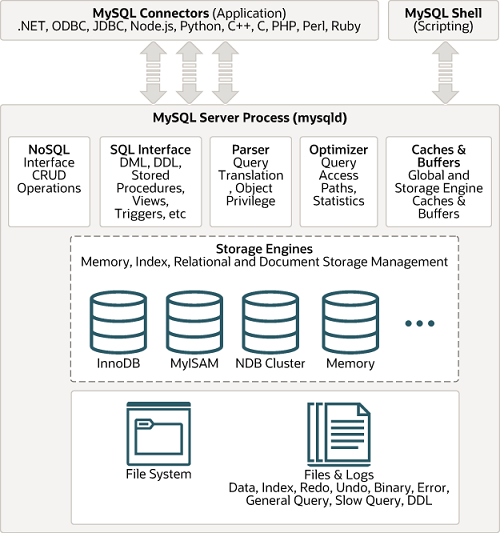
\includegraphics[width=0.7\linewidth]{includes/figures/mysql-architecture.png}
    \end{center}
\end{example}